\documentclass{article}

% PACKAGES
\usepackage[english]{babel}
\usepackage[T1]{fontenc}
\usepackage[letterpaper,top=1.5cm,bottom=1.5cm,left=3cm,right=3cm,marginparwidth=1.75cm]{geometry}
\usepackage{minted}
\usepackage{amsmath}
\usepackage{hyperref}
\usepackage{titlesec}
\usepackage{tocloft}
\usepackage{graphicx}
\usepackage[utf8]{inputenc}
\usepackage{array}
\usepackage{multirow}

% SETUP
\title{Projekt 2 - sortowanie}
\author{Aleksander Dygon - 151856}
\date{}

% table of contents links
\hypersetup{
    colorlinks = true,
    linkcolor = black
}

% domain range command, usage: \ci{start}{end}
\newcommand{\ci}[2]{\langle #1, #2 \rangle}

% space command, usage: \spa
\newcommand{\spa}[0]{\vspace{32pt}}

% paragraph command, usage \p{text}
\newcommand{\p}[1]{\paragraph{#1}\mbox{}\\}

% dots in chapters in table of contents
\renewcommand{\cftsecleader}{\cftdotfill{\cftdotsep}}

% DOCUMENT BEGIN
\begin{document}


\maketitle

\section*{Wstęp}
Celem tego projektu jest implementacja, przetestowanie i porównanie różnych metod sortowania tablic. W ramach projektu zostaną zbadane dwie grupy metod sortowania: I grupa metod - metody podstawowe (przez wstawianie, przez selekcję, sortowanie bąbelkowe) oraz II grupa metod - bardziej zaawansowane techniki sortowania (Quicksort, Sortowanie Shella, Sortowanie przez kopcowanie). Testy zostaną przeprowadzone na tablicach zawierających liczby całkowite z przedziału od -100 do 100.

\section*{Metody sortowania}
\subsection*{I grupa metod}
\begin{itemize}
    \item Przez wstawianie\\
    \textbf{Pseudokod:}
    \begin{verbatim}
    INSERTION-SORT(A)
        for j = 2 to A.length
            key = A[j]
            i = j - 1
            while i > 0 and A[i] > key
                A[i + 1] = A[i]
                i = i - 1
            A[i + 1] = key
    \end{verbatim}
    
    \item Przez selekcję\\
    \textbf{Pseudokod:}
    \begin{verbatim}
    SELECTION-SORT(A)
        for i = 1 to A.length - 1
            minIndex = i
            for j = i + 1 to A.length
                if A[j] < A[minIndex]
                    minIndex = j
            swap A[i] with A[minIndex]
    \end{verbatim}
    
    \item Sortowanie bąbelkowe\\
    \textbf{Pseudokod:}
    \begin{verbatim}
    BUBBLE-SORT(A)
        for i = 1 to A.length - 1
            for j = A.length downto i + 1
                if A[j] < A[j - 1]
                    swap A[j] with A[j - 1]
    \end{verbatim}
\end{itemize}

\subsection*{II grupa metod}
\begin{itemize}
    \item Quicksort\\
    \textbf{Pseudokod:}
    \begin{verbatim}
    QUICKSORT(A, p, r)
        if p < r
            q = PARTITION(A, p, r)
            QUICKSORT(A, p, q - 1)
            QUICKSORT(A, q + 1, r)
    
    PARTITION(A, p, r)
        x = A[r]
        i = p - 1
        for j = p to r - 1
            if A[j] <= x
                i = i + 1
                swap A[i] with A[j]
        swap A[i + 1] with A[r]
        return i + 1
    \end{verbatim}
    
    \item Sortowanie Shella\\
    \textbf{Pseudokod:}
    \begin{verbatim}
    SHELL-SORT(A)
        n = A.length
        gap = n / 2
        while gap > 0
            for i = gap to n - 1
                temp = A[i]
                j = i
                while j >= gap and A[j - gap] > temp
                    A[j] = A[j - gap]
                    j = j - gap
                A[j] = temp
            gap = gap / 2
    \end{verbatim}
    
    \item Sortowanie przez kopcowanie\\
    \textbf{Pseudokod:}
    \begin{verbatim}
    HEAPSORT(A)
        BUILD-MAX-HEAP(A)
        for i = A.length downto 2
            swap A[1] with A[i]
            A.heapSize = A.heapSize - 1
            MAX-HEAPIFY(A, 1)
    
    BUILD-MAX-HEAP(A)
        A.heapSize = A.length
        for i = floor(A.length / 2) downto 1
            MAX-HEAPIFY(A, i)
    
    MAX-HEAPIFY(A, i)
        left = 2i
        right = 2i + 1
        if left <= A.heapSize and A[left] > A[i]
            largest = left
        else largest = i
        if right <= A.heapSize and A[right] > A[largest]
            largest = right
        if largest != i
            swap A[i] with A[largest]
            MAX-HEAPIFY(A, largest)
    \end{verbatim}
\end{itemize}

\section*{Testy sortowania}
Sortowanie będzie testowane na trzech rodzajach danych wejściowych:
\begin{enumerate}
    \item Dla danych wygenerowanych losowo
    \item Dla danych posortowanych w kolejności odwrotnej (malejąco)
    \item Dla danych posortowanych właściwie (rosnąco)
\end{enumerate}

\subsection*{Dane wygenerowane losowo}
Wykres metod z grupy pierwszej:
\begin{figure}[H]
    \centering
    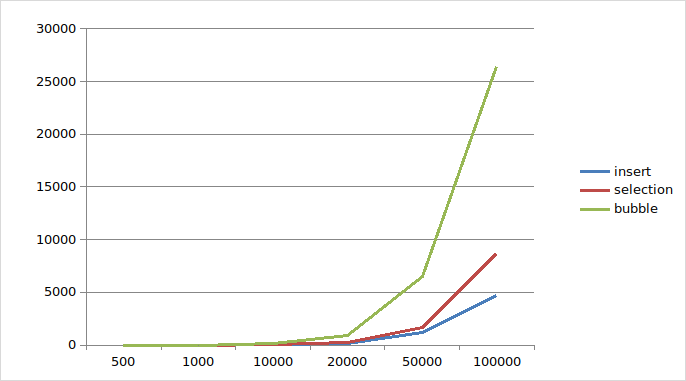
\includegraphics[width=\textwidth]{"../assets/1_1.png"}
    \label{fig:1_1}
\end{figure}


Wykres metod z grupy drugiej:
\begin{figure}[H]
    \centering
    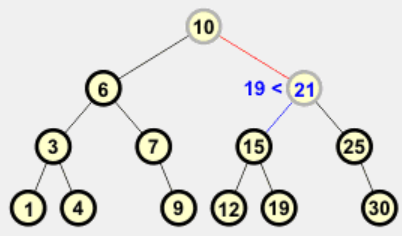
\includegraphics[width=\textwidth]{"../assets/1_2.png"}
    \label{fig:1_2}
\end{figure}

Wspólny wykres
\begin{figure}[H]
    \centering
    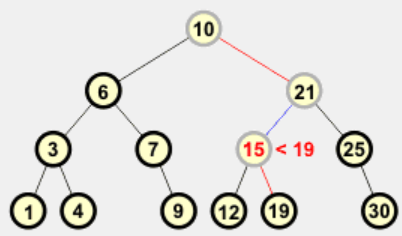
\includegraphics[width=\textwidth]{"../assets/1_3.png"}
    \label{fig:1_3}
\end{figure}
\subsection*{Dla danych posortowanych w kolejności odwrotnej (malejąco)}
Wykres metod z grupy pierwszej:
\begin{figure}[H]
    \centering
    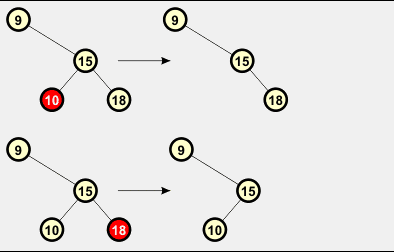
\includegraphics[width=\textwidth]{"../assets/2_1.png"}
    \label{fig:2_1}
\end{figure}


Wykres metod z grupy drugiej:
\begin{figure}[H]
    \centering
    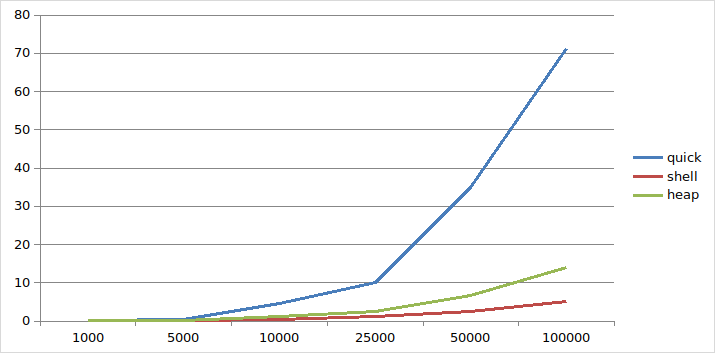
\includegraphics[width=\textwidth]{"../assets/2_2.png"}
    \label{fig:2_2}
\end{figure}

Wspólny wykres
\begin{figure}[H]
    \centering
    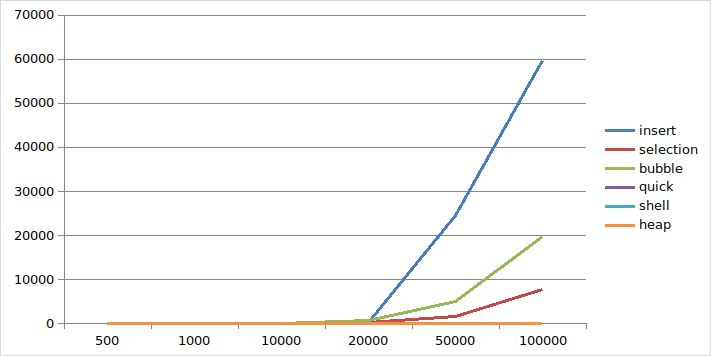
\includegraphics[width=\textwidth]{"../assets/2_3.png"}
    \label{fig:2_3}
\end{figure}
\subsection*{Dla danych posortowanych właściwie (rosnąco)}
Wykres metod z grupy pierwszej:
\begin{figure}[H]
    \centering
    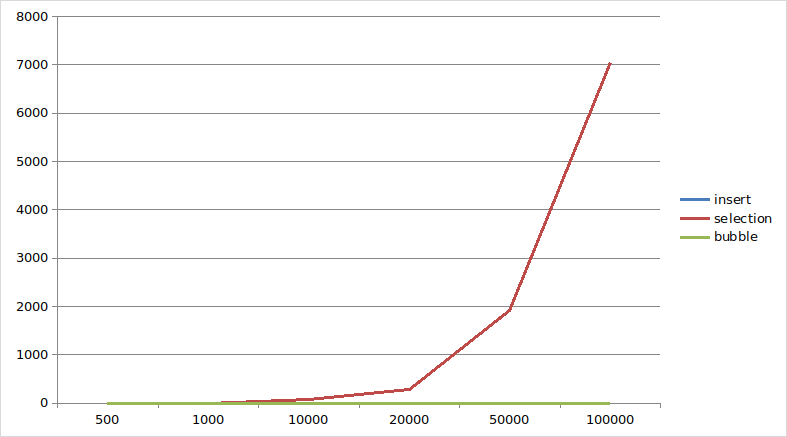
\includegraphics[width=\textwidth]{"../assets/3_1.png"}
    \label{fig:3_1}
\end{figure}


Wykres metod z grupy drugiej:
\begin{figure}[H]
    \centering
    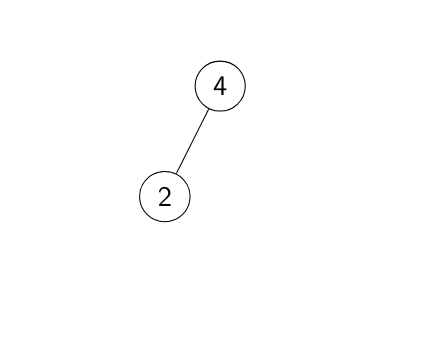
\includegraphics[width=\textwidth]{"../assets/3_2.png"}
    \label{fig:3_2}
\end{figure}

Wspólny wykres
\begin{figure}[H]
    \centering
    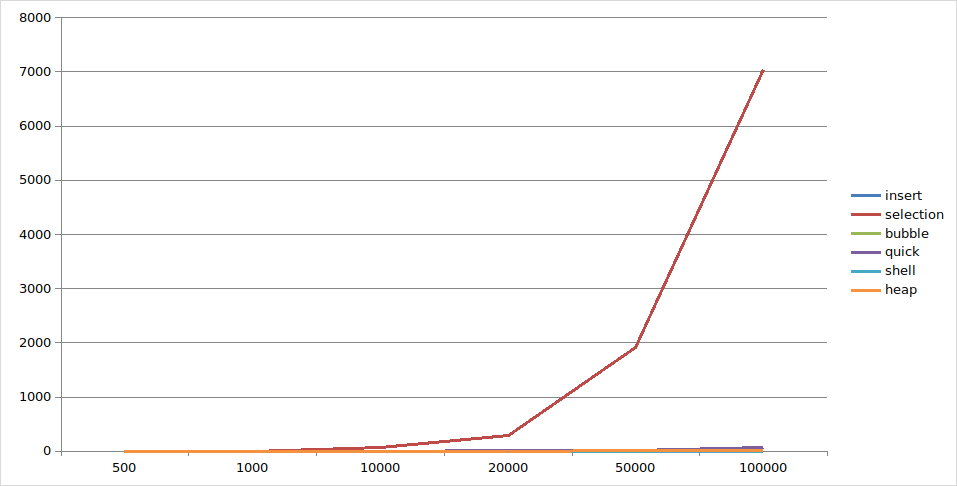
\includegraphics[width=\textwidth]{"../assets/3_3.png"}
    \label{fig:3_3}
\end{figure}

\subsection*{Tabelki Porównawcze}

Złozonosc obliczenia podanych metod sortowania \newline


\begin{table}[H]
    \begin{tabular}{lrlllll}
    n = 1000{[}ns{]} & \multicolumn{1}{l}{Bubble} & Selection                                   & Insertion                                   & Quicksort                                   & Heap                             & Shell                      \\
    Grupa I          & O(n\textasciicircum{}2)    & \multicolumn{1}{r}{O(n\textasciicircum{}2)} & \multicolumn{1}{r}{O(n\textasciicircum{}2)} & O(nlogn)                                    & O(nlogn) & O(n\textasciicircum{}1.14) \\
    Grupa II         & O(n\textasciicircum{}2)    & \multicolumn{1}{r}{O(n\textasciicircum{}2)} & \multicolumn{1}{r}{O(n\textasciicircum{}2)} & \multicolumn{1}{r}{O(n\textasciicircum{}2)} & O(nlogn) & O(n\textasciicircum{}1.14) \\
    Grupa III        & O(n\textasciicircum{}2)    & \multicolumn{1}{r}{O(n)}                    & \multicolumn{1}{r}{O(n)}                                       & \multicolumn{1}{r}{O(n\textasciicircum{}2)} & O(nlogn) & O(n\textasciicircum{}1.14)
    \end{tabular}
    \end{table}

BUBBLE 
\begin{table}[H]
    \begin{tabular}{lrlrlrlrlrlrl}
                       & \multicolumn{2}{l}{500}         & \multicolumn{2}{l}{1000}        & \multicolumn{2}{l}{10000}                                     & \multicolumn{2}{l}{20000}         & \multicolumn{2}{l}{50000}          & \multicolumn{2}{l}{100000}          \\
    \multirow{-2}{*}{} & \multicolumn{1}{l}{Exp} & Real  & \multicolumn{1}{l}{Exp} & Real  & \multicolumn{1}{l}{Exp}                             & Real    & \multicolumn{1}{l}{Exp} & Real    & \multicolumn{1}{l}{Exp} & Real     & \multicolumn{1}{l}{Exp} & Real      \\
    Grupa I            & 0,25                    & 0.432 & 1                       & 1.646 &  100  & 191.672 & 400                     & 895.818 & 2500                    & 6507.360 & 10000                   & 26426.420 \\
    Grupa II           & 0,25                    & 0.501 & 1                       & 2.218 &  100  & 205.695 & 400                     & 807.169 & 2500                    & 4985.443 & 10000                   & 19911.799 \\
    Grupa III          & 0,5                     & 0.003 & 0,001                   & 0.003 &  0,01 & 0.022   & 0,02                    & 0.045   & 0,05                    & 0.114    & 0,1                     & 0.223    
    \end{tabular}
    \end{table}
SELECTION

% Please add the following required packages to your document preamble:
% \usepackage{multirow}
\begin{table}[H]
    \begin{tabular}{lrlrlrlrlrlrl}
    \multirow{2}{*}{} & \multicolumn{2}{l}{500}         & \multicolumn{2}{l}{1000}        & \multicolumn{2}{l}{10000}        & \multicolumn{2}{l}{20000}         & \multicolumn{2}{l}{50000}          & \multicolumn{2}{l}{100000}         \\
                      & \multicolumn{1}{l}{Exp} & Real  & \multicolumn{1}{l}{Exp} & Real  & \multicolumn{1}{l}{Exp} & Real   & \multicolumn{1}{l}{Exp} & Real    & \multicolumn{1}{l}{Exp} & Real     & \multicolumn{1}{l}{Exp} & Real     \\
    Grupa I           & 0,25                    & 0.166 & 1                       & 0.873 & 100                     & 66.493 & 400                     & 292.711 & 2500                    & 1640.540 & 10000                   & 8725.437 \\
    Grupa II          & 0,25                    & 0.198 & 1                       & 0.958 & 100                     & 73.905 & 400                     & 326.040 & 2500                    & 1672.928 & 10000                   & 7869.311 \\
    Grupa III         & 0,25                    & 0.167 & 1                       & 0.659 & 100                     & 73.139 & 400                     & 294.170 & 2500                    & 1911.621 & 10000                   & 7048.667
    \end{tabular}
    \end{table}

INSERTION

% Please add the following required packages to your document preamble:
% \usepackage{multirow}
% \usepackage[table,xcdraw]{xcolor}
% Beamer presentation requires \usepackage{colortbl} instead of \usepackage[table,xcdraw]{xcolor}
\begin{table}[H]
    \begin{tabular}{lrlrlrlrlrlrl}
                       & \multicolumn{2}{l}{500}         & \multicolumn{2}{l}{1000}        & \multicolumn{2}{l}{10000}              & \multicolumn{2}{l}{20000}         & \multicolumn{2}{l}{50000}          & \multicolumn{2}{l}{100000}         \\
    \multirow{-2}{*}{} & \multicolumn{1}{l}{Exp} & Real  & \multicolumn{1}{l}{Exp} & Real  & \multicolumn{1}{l}{Exp}      & Real    & \multicolumn{1}{l}{Exp} & Real    & \multicolumn{1}{l}{Exp} & Real     & \multicolumn{1}{l}{Exp} & Real     \\
    Grupa I            & 0,25                    & 0.254 & 1                       & 0.525 & 100  & 91.392  & 400                     & 180.952 & 2500                    & 1199.758 & 10000                   & 4684.442 \\
    Grupa II           & 0,25                    & 0.501 & 1                       & 0.898 & 100  & 205.695 & 400                     & 381.383 & 2500                    & 24540.28 & 10000                   & 9633.041 \\
    Grupa III          & 0,5                     & 0.004 & 0,001                   & 0.004 & 0,01 & 0.038   & 0,02                    & 0.059   & 0,05                    & 0.134    & 0,1                     & 0.268   
    \end{tabular}
    \end{table}

QUICKSORT

% Please add the following required packages to your document preamble:
% \usepackage{multirow}
% \usepackage[table,xcdraw]{xcolor}
% Beamer presentation requires \usepackage{colortbl} instead of \usepackage[table,xcdraw]{xcolor}
\begin{table}[H]
    \begin{tabular}{lrlrlrlrlrlrl}
                       & \multicolumn{2}{l}{500}         & \multicolumn{2}{l}{1000}        & \multicolumn{2}{l}{10000}            & \multicolumn{2}{l}{20000}         & \multicolumn{2}{l}{50000}          & \multicolumn{2}{l}{100000}         \\
    \multirow{-2}{*}{} & \multicolumn{1}{l}{Exp} & Real  & \multicolumn{1}{l}{Exp} & Real  & \multicolumn{1}{l}{Exp}     & Real   & \multicolumn{1}{l}{Exp} & Real    & \multicolumn{1}{l}{Exp} & Real     & \multicolumn{1}{l}{Exp} & Real     \\
    Grupa I            & 0,0013                  & 0.029 & 0,003                   & 0.070 & 0,04                        & 0.981  & 0,0860                  & 2.169   & 0,2349                  & 9.433    & 0,5                     & 31.967   \\
    Grupa II           & 0,25                    & 0.198 & 1                       & 0.958 & 100 & 73.905 & 400                     & 326.040 & 2500                    & 1672.928 & 10000                   & 7869.311 \\
    Grupa III          & 0,25                    & 0.167 & 1                       & 0.659 & 100 & 73.139 & 400                     & 294.170 & 2500                    & 1911.621 & 10000                   & 7048.667
    \end{tabular}
    \end{table}

HEAP

% Please add the following required packages to your document preamble:
% \usepackage{multirow}
% \usepackage[table,xcdraw]{xcolor}
% Beamer presentation requires \usepackage{colortbl} instead of \usepackage[table,xcdraw]{xcolor}
\begin{table}[H]
    \begin{tabular}{lrlrlrlrlrlrl}
                       & \multicolumn{2}{l}{500}         & \multicolumn{2}{l}{1000}        & \multicolumn{2}{l}{10000}            & \multicolumn{2}{l}{20000}       & \multicolumn{2}{l}{50000}       & \multicolumn{2}{l}{100000}       \\
    \multirow{-2}{*}{} & \multicolumn{1}{l}{Exp} & Real  & \multicolumn{1}{l}{Exp} & Real  & \multicolumn{1}{l}{Exp}      & Real  & \multicolumn{1}{l}{Exp} & Real  & \multicolumn{1}{l}{Exp} & Real  & \multicolumn{1}{l}{Exp} & Real   \\
    Grupa I            & 0,0013                  & 0.050 & 0,003                   & 0.110 & 0,04 & 1.797 & 0,0860                  & 3.028 & 0,2349                  & 8.091 & 0,5                     & 16.917 \\
    Grupa II           & 0,0013                  & 0.046 & 0,003                   & 0.103 & 0,04 & 1.170 & 0,0860                  & 2.461 & 0,2349                  & 6.660 & 0,5                     & 14.030 \\
    Grupa III          & 0,0013                  & 0.069 & 0,003                   & 0.098 & 0,04 & 1.144 & 0,0860                  & 2.359 & 0,2349                  & 6.387 & 0,5                     & 13.261
    \end{tabular}
    \end{table}

SHELL

% Please add the following required packages to your document preamble:
% \usepackage{multirow}
% \usepackage[table,xcdraw]{xcolor}
% Beamer presentation requires \usepackage{colortbl} instead of \usepackage[table,xcdraw]{xcolor}
\begin{table}[H]
    \begin{tabular}{lrlrlrlrlrlrl}
                       & \multicolumn{2}{l}{500}         & \multicolumn{2}{l}{1000}        & \multicolumn{2}{l}{10000}              & \multicolumn{2}{l}{20000}       & \multicolumn{2}{l}{50000}       & \multicolumn{2}{l}{100000}       \\
    \multirow{-2}{*}{} & \multicolumn{1}{l}{Exp} & Real  & \multicolumn{1}{l}{Exp} & Real  & \multicolumn{1}{l}{Exp}        & Real  & \multicolumn{1}{l}{Exp} & Real  & \multicolumn{1}{l}{Exp} & Real  & \multicolumn{1}{l}{Exp} & Real   \\
    Grupa I            & 0,0012                  & 0.038 & 0,0026                  & 0.083 & 0,0363 & 1.292 & 0,0800                  & 2.322 & 0,2274                  & 6.168 & 0,5012                  & 12.660 \\
    Grupa II           & 0,0012                  & 0.019 & 0,0026                  & 0.038 & 0,0363 & 0.471 & 0,0800                  & 1.118 & 0,2274                  & 2.472 & 0,5012                  & 5.127  \\
    Grupa III          & 0,0012                  & 0.012 & 0,0026                  & 0.024 & 0,0363 & 0.340 & 0,0800                  & 0.731 & 0,2274                  & 2.095 & 0,5012                  & 4.215 
    \end{tabular}
    \end{table}
\section*{Podsumowanie}


Algorytmy o złożoności $O(n^2)$ (INSERT, SELECTION, BUBBLE) są wyraźnie nieefektywne dla dużych zbiorów danych, co widać po gwałtownym wzroście czasu wykonania. \newline
Quick Sort i Heap Sort są najbardziej efektywnymi algorytmami w analizie, szczególnie przy dużych zbiorach danych. \newline
Shell Sort oferuje dobrą wydajność i może być preferowanym wyborem w przypadkach, gdzie stabilność czasu wykonania jest istotna, choć nie dorównuje efektywnością Quick Sort i Heap Sort. \newline
Bubble Sort należy unikać w przypadku jakichkolwiek większych zbiorów danych z uwagi na ekstremalnie wysokie czasy wykonania. \newline


\end{document}